\chapter{Cadre et Contexte du travail}
\section*{Introduction}
Ce premier chapitre a pour objectif de contextualiser le projet dans son ensemble. Nous débutons par une présentation de l'organisme d'accueil. Ensuite, nous analysons la problématique actuelle en mettant en avant les limites et les difficultés rencontrées. Par la suite, nous proposons une solution adéquate. Enfin, nous concluons par une présentation de la méthodologie employée dans notre travail.
% Une section
\section{Organisme d'accueil}
Cette section est consacré pour la description de l’organisme d’accueil lors de notre stage PFE, nous présentons également les services qu’il propose à ses clients. 

\subsection{Présentation Générale}
Notre projet de fin d’études est mené au sein de Luceor Labs, un fournisseur de réseaux IP sans file. L'entreprise a été fondée en 2005 et rachetée par le groupe Novatel en 2021, ce qui lui a permis de se doter d'un cadre technologique plus solide et plus innovant. C'est une société mondiale dont le siège se trouve à Paris et qui est présente en Europe, au Moyen-Orient et en Afrique.

\subsection{Services et clients cibles}
 Luceor Labs fournit des équipements de réseau sans fil, des packs de gestion logicielle et des solutions avancées de bout en bout. 
Pour les organisations ayant des besoins de connectivité spécialisés, les produits Luceor simplifient la prise de décision et permettent la meilleure combinaison de couverture, de bande passante, de confidentialité et de sécurité. En outre, l'entreprise s'engage à fournir des solutions de communication de pointe aux clients qui opèrent dans des environnements exigeants où la sécurité et la fiabilité sont primordiales. Elle accompagne un large éventail de clients. Ces clients sont :

\begin{itemize}
    \item Les opérateurs d'entrepôts industriels et d'usines de marchandises ou de conteneurs
    \item Les institutions de sécurité publique
    \item Les responsables de la sécurité des événements
    \item Les sociétés minières
    \item Les Compagnies pétrolières et gazières
\end{itemize}

\section{Problématique}
La mise en œuvre de tout projet doit être précédée d'une analyse approfondie de la problématique, soulignant les points faibles du système actuel et les difficultés rencontrées. Actuellement, Luceor utilise l'application "StreamWide Team On Mission" pour les communications lors des missions internes et des opérations critiques, ce qui facilite la coordination des tâches entre les membres de l'équipe. Cet outil nous offre une solution complète de gestion de communication, avec un accent particulier sur les fonctionnalités spécifiques aux missions critiques et sur la sécurité des données. Cependant, son coût élevé pousse l'entreprise à envisager le développement d'une solution interne plus abordable, basée sur le serveur Asterisk. La société souhaite disposer des fonctionnalités minimales d'un service de communications critiques, telles que les appels audio et vidéo, ainsi que l'intégration avec sa propre base de données. Lors de la phase de développement, le manque d'un mécanisme automatisé pour gérer les versions exécutables du code peut causer des problèmes de gestion et ralentir la mise en production du produit. De plus, l'absence d'automatisation dans l'approvisionnement de l'infrastructure oblige les développeurs à créer manuellement les ressources du serveur, ce qui est plus chronophage comparé à l'utilisation d'un script déployable en une simple commande. L'absence de ce processus nous empêche de redémarrer rapidement l'environnement en cas de défaillance. Finalement, la connexion au serveur nécessite une application cliente SIP open-source.

\section[Solution proposée]{Solution proposée}
Pour résoudre le problème mentionné précédemment, nous allons implémenter un serveur Asterik. Ce serveur doit être déployé automatiquement sur une infrastructure cloud public comme AWS. L'objectif de l'utilisation du cloud est de rendre le serveur accessible à l'équipe de développement, libérant ainsi les développeurs des contraintes du travail en local et facilitant la communication des clients distants à travers différents réseaux.
De plus, l'utilisation d'une infrastructure en tant que code (IaC) nous permet d'allouer des ressources AWS comme une instance ubuntu EC2 et un dépot ECR de stockage des conteneurs. L'automatisation de création de notre propre infrastructure s'appuie sur Terraform comme outil d'IaC.  Après l'approvisionnement de l'infrastructure, notre solution doit inclure un pipeline CI/CD à travers GitHub Actions pour gérer la construction de notre serveur Asterisk et automatiser son déploiement dans l'instance EC2 comme étant un environnement de pré-production. Ce pipeline se déclenche à chaque fois que du code est livré sur l'outil de gestion des versions GitHub, dès qu'il y a des modifications. Cela assure une synchronisation efficace des codes sources et renforce la continuité offerte par l'approche DevOps. Le pipeline comprend deux phases. La première consiste à développer un processus de création d'une version exécutable pour Asterisk moyannant Dockerfile. Ensuite, nous stockons cette image dans le service de stockage des conteneurs ECR d’ AWS. La deuxième phase concerne le déploiement du serveur sur le cloud en utilisant l'image Docker stockée dans notre répertoire ECR. Durant cette phase, nous devons également lancer le service Asterisk avec un serveur base de données MySQL en utilisant Docker-Compose.
Une fois le pipeline est terminé avec succès, nous pouvons tester et effectuer des appels avec une application client SIP open-source. Linphone s'avère être la meilleure option, et nous envisageons de la personnaliser par la suite.
La figure \ref{fig:archi} illustre l'architecture de notre solution.
\begin{figure}[H]
        \centering
       \frame{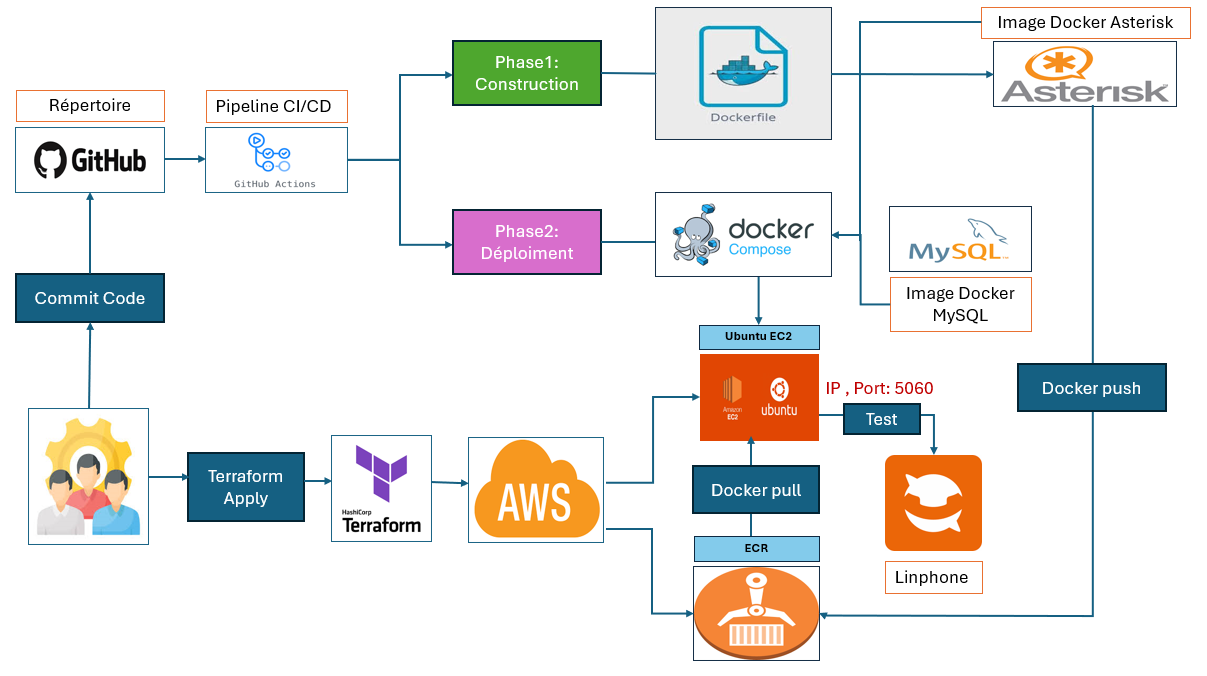
\includegraphics[width=17cm, height=12cm]{img/archi1.PNG}}
        \caption{Architecture de la solution proposée.}
        \label{fig:archi}
\end{figure}
        
Le passage à cette solution permet à l'entreprise de mieux maîtriser ses coûts, d'adapter l'outil à ses besoins spécifiques, et d'automatiser efficacement l'intégration et le déploiement de notre système de communication.

\section[Méthodologie de travail]{Méthodologie de travail}
Parmi les indispensables phases d’un projet, la définition d'une méthodologie de travail.

\subsection{Gestion de projet}
Pour garantir le bon déroulement de notre projet, nous adoptons la méthode Scrum. En effet, Scrum présente un cadre adapté pour gérer notre travail de manière efficace. Cette Méthodologie favorise la simplicité, l'agilité et la collaboration. De plus, elle vise à fixer la liste des tâches à effectuer en estimant pour chacune d’elle la durée de sa réalisation. Cela garantit la livraison d'un produit de haute qualité.

\subsection{Backlog du produit}
Dans cette section, nous présentons le backlog du produit (Product Backlog) qui est un élément crucial dans Scrum. Il sert à définir, organiser et prioriser les tâches à développer comme illustré dans le tableau \ref{tab:product_backlog}.

\begin{table}[h!]
    \centering
    \caption{Backlog du produit.}
    \begin{tabular}{|>{\centering\arraybackslash}m{1cm}|>{\centering\arraybackslash}m{3.5cm}|>{\centering\arraybackslash}m{4.5cm}|>{\centering\arraybackslash}m{1.5cm}|>{\centering\arraybackslash}m{2cm}|>{\centering\arraybackslash}m{2cm}|}
        \hline
        \textbf{ID} & \textbf{User Story} & \textbf{Description} & \textbf{Priorité} & \textbf{Difficulté} & \textbf{Durée} \\
        \hline
        1 & Étude comparative des outils DevOps & Réaliser une étude comparative des outils disponibles sur le marché afin d'identifier l'outil adapté & 3 & Moyenne & 2 semaines \\
        \hline
        2 & Implémentation d'une infrastructure & Implémenter une infrastructure cloud automatisée pour le déploiement de notre solution & 2 & Haute & 5 semaines \\
        \hline
        3 & Mise en place d'un pipeline CI/CD & Mettre en place une approche d'intégration et de déploiement continus en fonction des outils DevOps sélectionnés lors de l'étude comparative & 1 & Haute & 6 semaines \\
        \hline
        4 & Mise en place d'une configuration client-serveur & Mettre en place la configuration nécessaire pour établir une connexion client-serveur & 4 & Haute & 3 semaines \\
        \hline
    \end{tabular}
    \label{tab:product_backlog}
\end{table}

\section*{Conclusion}
Dans ce chapitre, nous avons traité le cadre général du projet, analysé la situation actuelle et la problématique, proposé une solution adéquate, et défini la méthodologie adoptée pour la réalisation de notre projet. Le chapitre suivant présentera un état de l'art sur les concepts fondamentaux de DevOps et du Cloud Computing. Nous y inclurons également une étude comparative des outils et technologies qui seront utilisés pour mettre en œuvre la solution.
% \chapter{Cadre et Contexte du travail}
% \section*{Introduction}
% Ce premier chapitre a pour objectif de contextualiser le projet dans son ensemble. Nous débutons par une présentation de l'organisme d'accueil. Ensuite, nous analysons la problématique actuelle en mettant en avant les limites et les difficultés rencontrées. Par la suite, nous proposons une solution adéquate. Enfin, nous concluons par une présentation de la méthodologie employée dans notre travail.
% % Une section
% \section{Organisme d'accueil}
% Cette section est consacré pour la description de l’organisme d’accueil lors de notre stage PFE, nous présentons également les services qu’il propose à ses clients. 

% \subsection{Présentation Générale}
% Notre projet de fin d’études est mené au sein de Luceor Labs, un fournisseur de réseaux IP sans file. L'entreprise a été fondée en 2005 et rachetée par le groupe Novatel en 2021, ce qui lui a permis de se doter d'un cadre technologique plus solide et plus innovant. C'est une société mondiale dont le siège se trouve à Paris et qui est présente en Europe, au Moyen-Orient et en Afrique.

% \subsection{Services et clients cibles}
%  Luceor Labs fournit des équipements de réseau sans fil, des packs de gestion logicielle et des solutions avancées de bout en bout. 
% Pour les organisations ayant des besoins de connectivité spécialisés, les produits Luceor simplifient la prise de décision et permettent la meilleure combinaison de couverture, de bande passante, de confidentialité et de sécurité. En outre, l'entreprise s'engage à fournir des solutions de communication de pointe aux clients qui opèrent dans des environnements exigeants où la sécurité et la fiabilité sont primordiales. Elle accompagne un large éventail de clients. Ces clients sont :

% \begin{itemize}
%     \item Les opérateurs d'entrepôts industriels et d'usines de marchandises ou de conteneurs
%     \item Les institutions de sécurité publique
%     \item Les responsables de la sécurité des événements
%     \item Les sociétés minières
%     \item Les Compagnies pétrolières et gazières
% \end{itemize}

% \section{Problématique}
% La mise en œuvre de tout projet doit être précédée d'une analyse approfondie de la problématique, soulignant les points faibles du système actuel et les difficultés rencontrées. Actuellement, Luceor utilise l'application "StreamWide Team On Mission" pour les communications lors des missions internes et des opérations critiques, ce qui facilite la coordination des tâches entre les membres de l'équipe. Cet outil nous offre une solution complète de gestion de communication, avec un accent particulier sur les fonctionnalités spécifiques aux missions critiques et sur la sécurité des données. Cependant, son coût élevé pousse l'entreprise à envisager le développement d'une solution interne plus abordable, basée sur le serveur Asterisk. La société souhaite disposer des fonctionnalités minimales d'un service de communications critiques, telles que les appels audio et vidéo, ainsi que l'intégration avec sa propre base de données. Lors de la phase de développement, le manque d'un mécanisme automatisé pour gérer les versions exécutables du code peut causer des problèmes de gestion et ralentir la mise en production du produit. De plus, l'absence d'automatisation dans l'approvisionnement de l'infrastructure oblige les développeurs à créer manuellement les ressources du serveur, ce qui est plus chronophage comparé à l'utilisation d'un script déployable en une simple commande. L'absence de ce processus nous empêche de redémarrer rapidement l'environnement en cas de défaillance. Finalement, la connexion au serveur nécessite une application cliente SIP open-source.

% \section[Solution proposée]{Solution proposée}
% Pour résoudre le problème mentionné précédemment, nous allons implémenter un serveur Asterik. Ce serveur doit être déployé automatiquement sur une infrastructure cloud public comme AWS. L'objectif de l'utilisation du cloud est de rendre le serveur accessible à l'équipe de développement, libérant ainsi les développeurs des contraintes du travail en local et facilitant la communication des clients distants à travers différents réseaux.
% De plus, l'utilisation d'une infrastructure en tant que code (IaC) nous permet d'allouer des ressources AWS comme une instance ubuntu EC2 et un dépot ECR de stockage des conteneurs. L'automatisation de création de notre propre infrastructure s'appuie sur Terraform comme outil d'IaC.  Après l'approvisionnement de l'infrastructure, notre solution doit inclure un pipeline CI/CD à travers GitHub Actions pour gérer la construction de notre serveur Asterisk et automatiser son déploiement dans l'instance EC2 comme étant un environnement de pré-production. Ce pipeline se déclenche à chaque fois que du code est livré sur l'outil de gestion des versions GitHub, dès qu'il y a des modifications. Cela assure une synchronisation efficace des codes sources et renforce la continuité offerte par l'approche DevOps. Le pipeline comprend deux phases. La première consiste à développer un processus de création d'une version exécutable pour Asterisk moyannant Dockerfile. Ensuite, nous stockons cette image dans le service de stockage des conteneurs ECR d’ AWS. La deuxième phase concerne le déploiement du serveur sur le cloud en utilisant l'image Docker stockée dans notre répertoire ECR. Durant cette phase, nous devons également lancer le service Asterisk avec un serveur base de données MySQL en utilisant Docker-Compose.
% Une fois le pipeline est terminé avec succès, nous pouvons tester et effectuer des appels avec une application client SIP open-source. Linphone s'avère être la meilleure option, et nous envisageons de la personnaliser par la suite.
% La figure \ref{fig:archi} illustre l'architecture de notre solution dont nous avons mentionné tous les outils et technologies nécessaire pour sa mise en place.
% \begin{figure}[H]
%         \centering
%        \frame{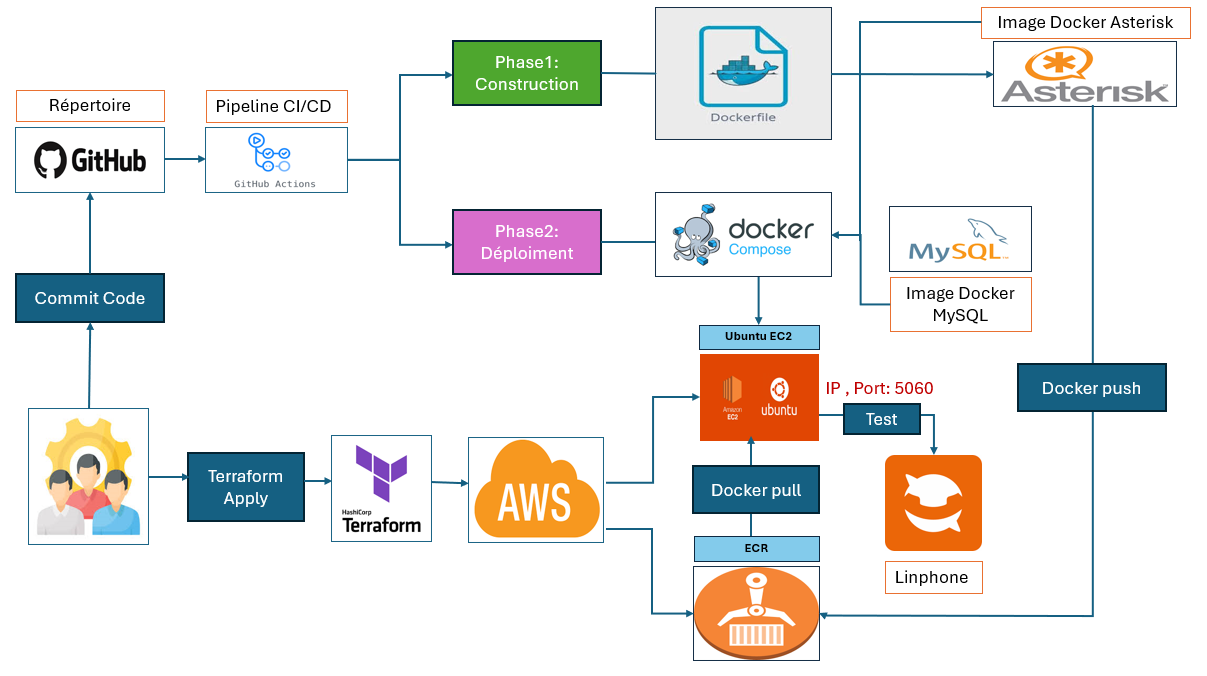
\includegraphics[width=17cm, height=10cm]{img/archi1.PNG}}
%         \caption{Architecture de la solution proposée.}
%         \label{fig:archi}
% \end{figure}
        
% Le passage à cette solution permet à l'entreprise de mieux maîtriser ses coûts, d'adapter l'outil à ses besoins spécifiques, et d'automatiser efficacement l'intégration et le déploiement de notre système de communication.

% \section[Méthodologie de travail]{Méthodologie de travail}
% \subsection{Gestion de projet}
% Pour garantir le bon déroulement de notre projet, nous adoptons la méthode Scrum. En effet, Scrum présente un cadre adapté pour gérer notre travail de manière efficace. Cette Méthodologie favorise la simplicité, l'agilité et la collaboration. De plus, elle vise à fixer la liste des tâches à effectuer en estimant pour chacune d’elle la durée de sa réalisation. Cela garantit la livraison d'un produit de haute qualité.
% \begin{table}
%     \centering
%     \caption{Backlog du produit.}
%     \begin{tabular}{|>{\centering\arraybackslash}m{1cm}|>{\centering\arraybackslash}m{3cm}|>{\centering\arraybackslash}m{5cm}|>{\centering\arraybackslash}m{1.5cm}|>{\centering\arraybackslash}m{2cm}|>{\centering\arraybackslash}m{2cm}|}
%         \hline
%         \textbf{ID} & \textbf{User Story} & \textbf{Description} & \textbf{Priorité} & \textbf{Difficulté} & \textbf{Durée} \\
%         \hline
%         1 & Étude comparative des outils DevOps & Réaliser une étude comparative des outils disponibles sur le marché afin d'identifier l'outil adapté & 3 & Moyenne & 2 semaines \\
%         \hline
%         2 & Implémentation d'une infrastructure & Implémenter une infrastructure cloud automatisée pour le déploiement de notre solution & 2 & Haute & 5 semaines \\
%         \hline
%         3 & Mise en place d'un pipeline CI/CD & Mettre en place une approche d'intégration et de déploiement continus en fonction des outils DevOps sélectionnés lors de l'étude comparative & 1 & Haute & 6 semaines \\
%         \hline
%         4 & Mise en place d'une configuration client-serveur & Mettre en place la configuration nécessaire pour établir une connexion client-serveur & 4 & Haute & 3 semaines \\
%         \hline
%     \end{tabular}
%     \label{tab:product_backlog}
% \end{table}

% \subsection{Backlog du produit}
% Dans cette section, nous présentons le backlog du produit (Product Backlog) qui est un élément crucial dans Scrum. Il sert à définir, organiser et prioriser les tâches à développer comme illustré dans le tableau \ref{tab:product_backlog}.



% \section*{Conclusion}
% Dans ce chapitre, nous avons traité le cadre général du projet, analysé la situation actuelle et la problématique, proposé une solution adéquate, et défini la méthodologie adoptée pour la réalisation de notre projet. Le chapitre suivant présentera un état de l'art sur les concepts fondamentaux de DevOps et du Cloud Computing. Nous y inclurons également une étude comparative des outils et technologies qui seront utilisés pour mettre en œuvre la solution.
